\chapter{Methods}
\section{Latest updates - TD2C}
As said in \ref{introd2c}, D2C was introduced in \cite{bontempi2015dependency}. Later on, with \cite{bontempi2020learning} and \textbf{\cite{TD2C paper}}, certain aspects of the original procedure have been changed to solve some of the problematics (e.g. computational cost). \\

At firs, the authors introduced a new descriptor, aiming to featurize the context, based on the notion of interaction information: $$I(m^{(1)}_i;m^{(2)}_i;X_i) = I(m^{(1)};m^{(2)}_i;X_i) - I(m^{(1)}_i;m^{(2)}_i|X_i),$$ which gives insights on the causal links characterizing the considered data (in particular, positive interactions derive from common effect configurations, while negative ones form common cause configurations), in order to derive an appropriate DAG structure. The underlying context is maybe more clear in Figure \textbf{\textit{inserire figura}}, where given the latent nature of the nodes F and G, no d-separation (i.e. no independence) occurs between the nodes B,C,D,E and the node A. This means that the features associated to the nodes B,C,D,E are informative about the state of the node A. In other words, by measuring the quantities represented by nodes B,C,D,E we may reduce the uncertainty about the binary state of the node A. \textbf{\textit{figure3}}. As a result, the ranking procedure described in \ref{d2c} is simplified (no more bootstrapping is needed, instead, a correlation to the target measure is used), and complexity for each pair $X_i$ - $X_j$ becomes $O(Cn + K^2N)$.\\
This addition wanted to show that context aware learning approaches, as the ones based on Granger causality (methods based on the precedence concept, which is an associative measure not a causal one and so usually utilized to infer strong relevance and not causality), are adequate to infer causal relationships in large variate contexts, as for multivariate TS. This first modification is in \cite{bontempi2020learning} and is called caD2C ("context aware").\\

The last update (\textbf{\cite{TD2C paper}}) of the method proposes some variations to better leverage the temporal dependencies of time series data and reduce the dimensionality of the problem.
Starting from the same set of assumptions as before: absence of confounding, selection bias, and feedback configurations, faithfulness, stationarity and lagged effects ($X^{(t-1)}_i \rightarrow X^{(t)}_i \ \forall \ (i, t)$), it proposes the followings:
\begin{itemize}
    \item Thanks to the lagged effects assumption, it is able to reduce the relevant members of a considered MB, i.e. to reduce dimensionality, and so to skip the MB estimation phase of \cite{bontempi2015dependency}.
    Looking at the simplified example in Figure \ref{TS}, we see that, studying the causal link $X^{(t)}_i \rightarrow X^{(t+1)}_j$ and only considering effects and causes for them, we can reduce the asymmetric mixtures seen in Table \ref{table1} to the ones in Table \ref{table4} 
    \item Adopts the knnCMI method to estimate conditional mutual information using a nearest neighbors approach, differently from \cite{bontempi2020learning}, where a prediction error from a regression model was informing the entropy estimation under the Gaussian assumption.
    \item precise which descriptors are used
    \item precise all the data generating process and so how complexity changes
\end{itemize}

\begin{table}[!ht]
    \centering
    \caption{Shrinked set of descriptors used by TD2C}
    \begin{tabular}{c|c}
    \hline
        \textbf{CMI terms \ \ $\forall \ \ (m^{(k_i)}_i, m^{(k_j)}_j)$} & \textbf{Families of asymmetric mixtures} \\ \hline
        ~$I(X_i; m^{(k_j)}_j|X_j)$ & $D_{xmx}(i,j) = I(X^{(t)}_i; m^{(k_j)}_j|X^{(t+1)}_j)$, $m^{(k_j)}_j \in \{X^{(t+2/t)}\}$~ \\
        ~$I(X_j; m^{(k_i)}_i|X_i)$ & $D_{xmx}(j,i) = I(X^{(t+1)}_j; m^{(k_i)}_i|X^{(t)}_i)$, $m^{(k_i)}_i \in \{X^{(t-1/t+1)}\}$~ \\
        ~$I(m^{(k_i)}_i; m^{(k_j)}_j|X_i)$ & $D_{mmx}(i,j) = I(X^{(t-1/t+1)}_i; m^{(k_j)}_j|X^{(t)}_i)$, $m^{(k_j)}_j \in \{X^{(t/t+2)}\}$~ \\
        ~$I(m^{(k_j)}_j; m^{(k_i)}_i|X_j)$& $D_{mmx}(j,i) = I(X^{(t/t+2)}_j; m^{(k_i)}_i|X^{(t+1)}_j)$, $m^{(k_i)}_i \in \{X^{(t-1/t+1)}\}$~ \\ \hline
    \end{tabular}
    \label{table4}
\end{table}

The final algorithm procedure becomes: 
\begin{enumerate}
    \item Estimate the new reduced version of $MB_i$ and $MB_j$.
    \item Derive the set of descriptors and their empirical distributions' quantiles to create the input vectors ($d$) for the classifier.
    \item Label each input vector as causal ($1$) or non causal ($0$), to create the target variable ($y$).
    \item Classifier training based on the final dataset.
    \item Prediction on an unseen testset.
\end{enumerate}

\textbf{\textit{Insert the formalized algorithm}}.


\begin{figure}[!h]
  \centering
  \begin{tikzpicture}
  
    % NODES
    \node (graph) at (-1,4) {
      \begin{tikzpicture}
        \draw[thick] (0.5,0.5) -- (0.5,1.5) -- (2.5,1.5) -- (2.5,0.5) -- cycle;
        \node at (1.5,1) {DAG};
      \end{tikzpicture}
    };
    \node[text width=5cm, anchor=center, align=center] at (-1,6) {1. A preliminary DAG of the type \ref{TS} is created at random to initialize the process following some restriction (size, components, etc.)};

    \node (table3) at (-1,0) {
    \begin{tabular}{|c|c|}
        \hline
        Simulated data\\ \hline
        $X_{1,1}, X_{1,2}, ..., X_{1,n}$ \\ \hline
        $X_{2,1}, X_{2,2}, ..., X_{2,n}$ \\ \hline
        $...$ \\ \hline
        $X_{20,1}, X_{20,2}, ..., X_{20,n}$ \\
        \hline
      \end{tabular}
    };
    \node[text width=8cm, anchor=center, align=center] at (-1,-3) {2. From the preliminary DAG, data are generated using the generative processes (\ref{gp}). Data will be of the type \textbf{\textit{appendix for details}}};

    \node (table2a) at (7,3) {
        \begin{tabular}{|c|c|c|}
        \hline
        Relation & Descr. vector & Class\\ \hline
        $X_1 \rightarrow X_2$ & $(d_{1,1}, ..., d_{1,28})$ & 1\\ \hline
        $X_1 \rightarrow X_3$ & $(d_{2,1}, ..., d_{2,28})$ & 0 \\ \hline
        ... & ... & ... \\ \hline
        $X_m \rightarrow X_n$ & $(d_{m,1}, ..., d_{m,28})$ & 1 \\ 
        \hline
      \end{tabular}
    };
    \node[text width=9cm, anchor=center, align=center] at (7,6) {3. Descriptors (\ref{descriptors}) are computed for each couple of variables in the MB and a dataset made of descriptors vectors and class labels is formed};
    
\node (graph2) at (7,-0.5) {
      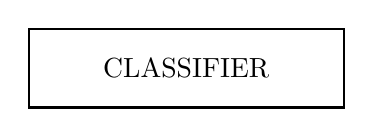
\begin{tikzpicture}
        \draw[thick] (0.5,0.5) -- (0.5,1.5) -- (4.5,1.5) -- (4.5,0.5) -- cycle;
        \node at (2.5,1) {CLASSIFIER};
      \end{tikzpicture}
    };
    \node[text width=7cm, anchor=center, align=center] at (7,-2) {4. The resulting dataset is given to a classifier \textbf{\textit{(refer to data analysis made to find the best classifier)}}};

    % ARROWS
    \draw[->, line width = 0.5mm] (table2a.south) -- (graph2.north);
    \draw[->, line width = 0.5mm] (table3.east) -- (table2a.west);
    \draw[->, line width = 0.5mm] (graph) -- (table3.north);

  \end{tikzpicture}
  
  \caption{D2C process}
  \label{proc}
\end{figure}

\subsection{Latest applications} \label{prev}
Let's take a look at some of the most relevant experiments conducted by previous studies, what they put the focus on, their methods and their results.\\

The three papers cited above (\cite{bontempi2015dependency}, \cite{bontempi2020learning} and \textbf{\textit{TD2C paper}}) are the lendmarks in D2C method's literature. To have a better look of what has been achieved so far can help us understand what could give a significant contribute to this method. Let's summarize what these three studies have concluded.\\

\textbf{\textit{(rephrase a little)}}\\
In \cite{bontempi2015dependency} the D2C algorithm was assessed using synthetic data, addressing the problem of inferring causal links from synthetic data generated for linear and non-linear DAG configurations of different sizes. The assessment procedure relied on the generation of a number of DAG structures and the simulation, for each of them, of N node observations according to the additive dependency relation $$x_i = \sum_{j \in par(i)} f_{i,j}(x_j) + e_i, \ \ i = 1, ..., n.$$ For each DAG, on the basis of its structure and the data set of observations, a number of pairs $<d, y>$, where $d$ is the descriptor vector and $y$ is the class denoting the existence (or not) of the causal link in the DAG topology, was collected. A Random Forest classifier was trained on the balanced data set. The test set was obtained by considering a number of independently simulated DAGs. This approach has then been compared in terms of classification accuracy (Balanced Error Rate (BER)) to several state-of-the-art approaches.
Some of the most relevant results were the following:
\begin{itemize}
    \item The improvement of D2C wrt state-of-the-art techniques (often based on linear assumptions) tends to increase when nonlinear configurations were used.
    \item The accuracy of the D2C approach improves by increasing the number of training examples.
    \item The analysis of the importance of the D2C descriptors showed that the most relevant variables for the method were only part of the ones considered in vector $d$.
\end{itemize}

In \cite{bontempi2020learning} ...\\

Finally, in \textbf{\textit{TD2C paper}} ...\\


\section{Contributions}
We try now to give our contribute to the analyzed methods, suggesting solutions to declared problems and limitations and/or simple changes that could improve them.\\

As we have seen in Section \ref{prev}, there are enough ideas to conduct interesting analyses. Here, we display all the contributions that this work tries to give to the method, based on the main limitations encountered so far by the previous studies. We divide them into five topics:
\begin{enumerate}
    \item Real-data validation (\ref{contr1})  
    \item Linear processes validation (\ref{contr2})
    \item TD2C extesions (\ref{contr3})
    \item Computational cost reduction (\ref{contr4}) 
    \item Code contributions (\ref{contr5})
\end{enumerate}

In each section, the conditions under which the experiments have been conducted are specified. The general setting is similar to the one specified in \textbf{\textit{TD2C paper}}, with some modifications useful to each specific goal. Python, Rstudio and Causeme softwares have been used.

\subsubsection{Real-data validation}
\textbf{\textit{[12-18/8 week]}}
As said before, real-data validation is missing in the three cited papers. Therefore, in this section we try to do it to see how TD2C could be applied in realistic scenarios and how its performances would behave.\\

\textbf{\textit{Explain why this is useful}}


\subsubsection{Linear processes validation} 
\textbf{\textit{[19-25/8 week]}} Looking at the generative processes (\ref{gp}) adopted by the method in the synthetic data generation step, we notice that (18), (19) and (20) are the only linear ones. 
Since the results has been obtained through LOPOCV (Leave-one-process-out cross-validation), we can state that, when it come the turn of one of those three linear processes to generate the testset data, results are, on average, worse than the other cases. This problematic gives use the input for some interesting questions that could help method's validation and applicability:\\
- How TD2C's performances would be if we generate data only from those three linear processes?\\
- How TD2C's performances would be if we generate data from a smaller (or biiger) number of processes, as has been done so far?\\
- How TD2C's performances would be if we generate data from a different pool of processes, possibly where the majority of them are linear?\\
Following these questions, different generative processes sets have been used to train the algorithm and the Causeme platform has been used to validate the resulting parameters.

\subsubsection{TD2C extesions}
\textbf{\textit{[26/8-1/9 week]}} In this section we report the most relevant purposes for effective innovations of TD2C method and their experimentation.\\

\textbf{Markov Blanket changes}\\ 
The first two purposes we tested for are linked to the concept of Markov Blanket (MB). Starting from the context in Figure \ref{TD2CMB},
\begin{figure}[!h]
\centering
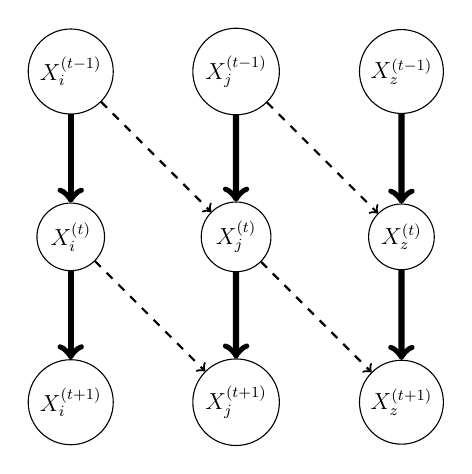
\begin{tikzpicture}[
  every node/.style={draw, circle, minimum size=1cm, font=\large}, % Reduced node size
  dashed edge/.style={draw,->,thick, dashed},
  solid edge/.style={draw,->,thick},
  scale=0.7, % Scale down the entire picture
  transform shape % Ensure scaling affects the whole picture
]
% Define the nodes
\node (A) at (0,2) {$X^{(t-1)}_i$};
\node (B) at (0,-1) {$X^{(t)}_i$};
\node (C) at (0,-4) {$X^{(t+1)}_i$};
\node (D) at (3,2) {$X^{(t-1)}_j$};
\node (E) at (3,-1) {$X^{(t)}_j$};
\node (F) at (3,-4) {$X^{(t+1)}_j$};
\node (G) at (6,2) {$X^{(t-1)}_z$};
\node (H) at (6,-1) {$X^{(t)}_z$};
\node (I) at (6,-4) {$X^{(t+1)}_z$};
% Define the edges
\path[solid edge, line width=0.8mm] (A) edge (B);
\path[solid edge, line width=0.8mm] (B) edge (C);
\path[solid edge, line width=0.8mm] (D) edge (E);
\path[solid edge, line width=0.8mm] (E) edge (F);
\path[solid edge, line width=0.8mm] (G) edge (H);
\path[solid edge, line width=0.8mm] (H) edge (I);
\path[dashed edge] (B) edge (F);
\path[dashed edge] (A) edge (E);
\path[dashed edge] (E) edge (I);
\path[dashed edge] (D) edge (H);
\end{tikzpicture}
\caption{An example of three time series displayed in a DAG, with the assumptions of no instantaneous effects, temporal effects and stationarity.}
\label{TD2CMB}
\end{figure}
we tried to consider a wider MB, by both going backwards, considering passed instants (Figure \ref{back}),

\begin{figure}[!h]
\centering
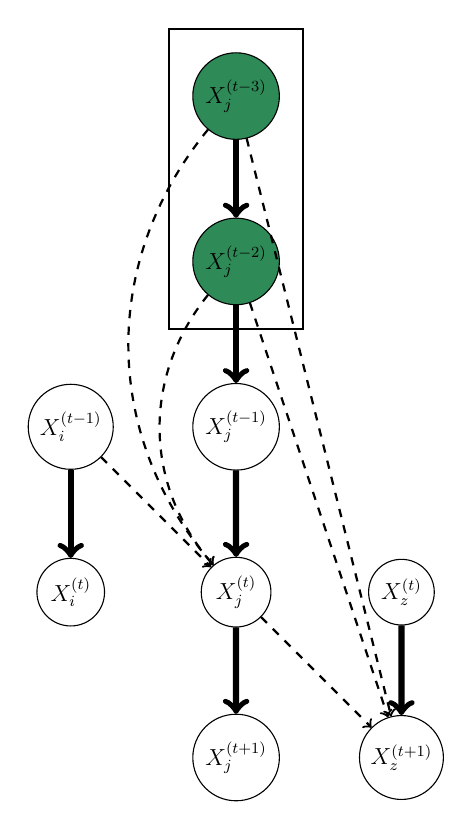
\begin{tikzpicture}[
  every node/.style={draw, circle, minimum size=1cm, font=\large}, % Reduced node size
  dashed edge/.style={draw,->,thick, dashed},
  solid edge/.style={draw,->,thick},
  scale=0.7, % Scale down the entire picture
  transform shape % Ensure scaling affects the whole picture
]

% Include the fit library
\usetikzlibrary{fit}

% Define the nodes
\node (A) at (0,2) {$X^{(t-1)}_i$};
\node (B) at (0,-1) {$X^{(t)}_i$};
\node (D) at (3,2) {$X^{(t-1)}_j$};
\node (E) at (3,-1) {$X^{(t)}_j$};
\node (F) at (3,-4) {$X^{(t+1)}_j$};
\node (H) at (6,-1) {$X^{(t)}_z$};
\node (I) at (6,-4) {$X^{(t+1)}_z$};
\node[fill = SeaGreen] (L) at (3,5) {$X^{(t-2)}_j$};
\node[fill = SeaGreen] (M) at (3,8) {$X^{(t-3)}_j$};

% Draw a black rectangle around nodes M and L
\node[draw, thick, rectangle, fit=(M) (L), inner sep=0.3cm] {};

% Define the edges
\path[solid edge, line width=0.8mm] (A) edge (B);
\path[solid edge, line width=0.8mm] (D) edge (E);
\path[solid edge, line width=0.8mm] (E) edge (F);
\path[solid edge, line width=0.8mm] (H) edge (I);
\path[solid edge, line width=0.8mm] (M) edge (L);
\path[solid edge, line width=0.8mm] (L) edge (D);
\path[dashed edge] (A) edge (E);
\path[dashed edge] (E) edge (I);
\path[dashed edge] (M) edge (I);
\path[dashed edge] (L) edge (I);
\path[dashed edge, bend right = 40] (M) edge (E);
\path[dashed edge, bend right = 40] (L) edge (E);
\end{tikzpicture}
\caption{An example of three time series displayed in a DAG, with the assumptions of no instantaneous effects, temporal effects and stationarity.}
\label{back}
\end{figure}
 and enlarging the number of variables by considering the MBs of the MB variables (Figure \ref{MBMB}), 
 \begin{figure}[!h]
\centering
\begin{tikzpicture}[
  every node/.style={draw, circle, minimum size=1cm, font=\large}, % Reduced node size
  dashed edge/.style={draw,->,thick, dashed},
  solid edge/.style={draw,->,thick},
  scale=0.7, % Scale down the entire picture
  transform shape % Ensure scaling affects the whole picture
]
% Define the nodes
\node[fill = Goldenrod] (Z) at (-3,2) {$Z_{t-1}$};
\node[fill = Goldenrod] (ZZ) at (-3,-1) {$Z_{t}$};
\node[fill = Goldenrod] (ZZZ) at (-3,-4) {$Z_{t+1}$};
\node[fill = Melon] (A) at (0,2) {$A_{t-1}$};
\node[fill = Melon] (AA) at (0,-1) {$A_{t}$};
\node[fill = Melon] (AAA) at (0,-4) {$A_{t+1}$};
\node[fill = WildStrawberry] (B) at (3,2) {$B_{t-1}$};
\node[fill = WildStrawberry] (BB) at (3,-1) {$B_{t}$};
\node[fill = WildStrawberry] (BBB) at (3,-4) {$B_{t+1}$};
\node[fill = WildStrawberry] (C) at (6,2) {$C_{t-1}$};
\node[fill = WildStrawberry] (CC) at (6,-1) {$C_{t}$};
\node[fill = WildStrawberry] (CCC) at (6,-4) {$C_{t+1}$};
\node[fill = Melon] (D) at (9,2) {$D_{t-1}$};
\node[fill = Melon] (DD) at (9,-1) {$D_{t}$};
\node[fill = Melon] (DDD) at (9,-4) {$D_{t+1}$};
\node[fill = Goldenrod] (E) at (12,2) {$E_{t-1}$};
\node[fill = Goldenrod] (EE) at (12,-1) {$E_{t}$};
\node[fill = Goldenrod] (EEE) at (12,-4) {$E_{t+1}$}
% Define the edges
\path[solid edge, line width=0.8mm] (A) edge (AA);
\path[solid edge, line width=0.8mm] (AA) edge (AAA);
\path[solid edge, line width=0.8mm] (B) edge (BB);
\path[solid edge, line width=0.8mm] (BB) edge (BBB);
\path[solid edge, line width=0.8mm] (C) edge (CC);
\path[solid edge, line width=0.8mm] (CC) edge (CCC);
\path[solid edge, line width=0.8mm] (D) edge (DD);
\path[solid edge, line width=0.8mm] (DD) edge (DDD);
\path[solid edge, line width=0.8mm] (E) edge (EE);
\path[solid edge, line width=0.8mm] (EE) edge (EEE);
\path[solid edge, line width=0.8mm] (Z) edge (ZZ);
\path[solid edge, line width=0.8mm] (ZZ) edge (ZZZ);
\path[dashed edge] (Z) edge (AA);
\path[dashed edge] (ZZ) edge (AAA);
\path[dashed edge] (A) edge (BB);
\path[dashed edge] (AA) edge (BBB);
\path[solid edge, color = red, line width=0.8mm] (B) edge (CC);
\path[solid edge, color = red, line width=0.8mm] (BB) edge (CCC);
\path[dashed edge] (C) edge (DD);
\path[dashed edge] (CC) edge (DDD);
\path[dashed edge] (D) edge (EE);
\path[dashed edge] (DD) edge (EEE);
\end{tikzpicture}
\caption{In red, the couple of variables whose causality's direction is the main goal (B and C), in orange, MB's variables for B and C (A and D) and, in yellow, MB's variables of A and D (Z and E)}
\label{MBMB}
\end{figure}
 eventually conditioning on more than one variable to build asymmetric relations. \\
 
\textbf{Iterative TD2C and TD2C helping}\\
The other two purposes take the method as it is and integrate it in different ways to obtain better results. The first one is the one we call iterative TD2C, it consists in iteratively running the method by taking the results as probabilities and using them in the subsequent iteration to better our knowledge on MB's associations. The last purpose is TD2C helping, where we use results from state of the art methods to reinforce our knowledge on the MB and then running TD2C starting from those premises (or viceversa, using TD2C as a starting point for other state of the art methods).

\subsubsection{Computational cost reduction}
\textbf{\textit{[2-8/9 week, we will see if this topic is too large to be included]}} One of the main limit for TD2C (as well as for D2C) is the elevated computational cost, also due to the sum of complexities through the different phases of the process, not just relatively to the algorithm itself. In \cite{bontempi2020learning} the original computational costs had been reduced by ... \textbf{\textit{summary of complexity analysis of previous papers}}... In order to reduce this costs we proposed some potential changes and we ran several experiments to verify their validity.\\
- Descriptors reduction (at this stage we also made a classifier selection): selection of the most relevant descriptors.\\
- Introduction of the Meek rules to reduce the couples of variable in the MB to be considered (\textit{The Meek Rules help complete the orientation of edges in a mixed graph, resulting in a CPDAG that reflects the possible causal relationships among variables while accounting for the observed conditional independencies in the data. The CPDAG is a more refined and directed version of the original PDAG (Partially Directed Acyclic Graph) obtained from the data.})\\


\subsubsection{Code contributions}
[In the meantime, so 12/8-15/9] This section wants to summarise all the contributions made relatively to the Python code of TD2C and show some results from the jupyter nootbooks that  have been created with the purpose of simplifying the application of the method for future users. Examples of useful notebooks: a notebook that makes easy the application of the method and of its functions; a notebook that simplifies the application of the method to real-data, ecc.

